\documentclass[10pt]{article}
\usepackage[margin=.9in]{geometry}
\usepackage{graphicx,booktabs,natbib,amsmath}
\usepackage[hidelinks]{hyperref}
\newcommand{\result}[2]{#2}
% [results-sha256:41aeaf8dd7080f2a4e2c0abc9646ed5fd46db730c4acb59993148a1bf9aa807a]
\title{A Descriptive Revisit of the U.S. Beveridge Curve, 2001--2024}
\author{Real-data research pilot}
\date{October 2026}
\begin{document}
\maketitle
\begin{abstract}
Using a frozen snapshot of 288 paired monthly U.S. labor-market observations from the Bureau of Labor Statistics (BLS), this note compares job-openings rates in months with similar unemployment rates before and after the pandemic transition. In the 3.5--4.5 percent unemployment interval, the mean openings rate was \result{primary.pre_mean}{4.10} percent in 2001--2019 and \result{primary.post_mean}{5.70} percent in 2022--2024, a descriptive gap of \result{primary.difference}{1.60} percentage points. The 2024-only gap was \result{last_year_check.difference_from_pre}{0.55} points. This is a reproducibility and workflow pilot of an already known pattern, not a novel or causal finding. Survey measurement, revisions, compositional change, serial dependence, and limited support restrict interpretation.
\end{abstract}

\section{Introduction}
% [claim:c-question]
The Beveridge curve plots vacancies against unemployment. BLS has long published precisely this comparison and documented outward movements in earlier periods \citep{BLS2013,BLSChart}. This note asks a narrow descriptive question: among months with comparable measured unemployment, how different were published U.S. job-openings rates in 2022--2024 relative to 2001--2019? The exercise tests an end-to-end research workflow using real government data, rather than proposing a new economic mechanism or claiming a contribution to the literature.

\section{Related Evidence}
% [claim:c-question]
BLS's earlier Beveridge-curve chart already reports time variation in the vacancy--unemployment relationship \citep{BLS2013}. The live BLS chart uses the same two aggregate rate series \citep{BLSChart}. \citet{BarlevyEtAl2023} analyze changing reasons for Beveridge-curve shifts through 2023, while \citet{KindbergGirard2024} study the pandemic shift with state data and a search model. Their scope and interpretation are much deeper than our two-period summary. Recent BLS work examines whether unusually high JOLTS openings after 2020 reflect reporting or processing error \citep{BLS2026}. Our arithmetic comparison neither supersedes those analyses nor resolves the mechanisms behind the joint movement. Its contribution is limited to an auditable real-data workflow demonstration.

\section{Data and Measurement}
% [data:bls-monthly-rates]
We retrieved the seasonally adjusted civilian unemployment rate (CPS series LNS14000000) and total nonfarm job-openings rate (JOLTS series JTS000000000000000JOR) directly from BLS Public Data API version 2.0 \citep{BLSAPI,BLSChart}. The snapshot contains monthly observations from January 2001 through December 2024: \result{sample.months_all}{288} months paired by year and month. The raw JSON bodies, timestamps, request windows, hashes, and acquisition script are in the research package. BLS describes a job opening as an unfilled position with available work, a start possible within 30 days, and active external recruitment \citep{BLSDefinitions}. The openings rate divides openings by employment plus openings. Both values are published aggregate estimates, not simulated observations or individual-level records.

The baseline is January 2001--December 2019 (\result{sample.baseline_months}{228} months); the comparison is January 2022--December 2024 (\result{sample.comparison_months}{36} months). We exclude the \result{sample.excluded_transition_months}{24} months of 2020--2021 from the comparison to avoid mixing acute pandemic and reopening observations into either window. This is an ex-post descriptive choice. No observations are missing in the retrieved paired series. BLS estimates can be revised; the frozen snapshot defines the replication target. BLS published material is public domain with requested attribution \citep{BLSCopyright}.

\section{Descriptive Design}
% [claim:c-design]
Let $U_t$ and $V_t$ denote published unemployment and openings rates. For an unemployment interval $I$, we compute
\[
\Delta(I)=\operatorname{mean}(V_t\mid t\in 2022{:}2024, U_t\in I)
-\operatorname{mean}(V_t\mid t\in 2001{:}2019, U_t\in I).
\]
The primary interval is $I=[3.5,4.5]$ percentage points, chosen to create common support across the two windows. A secondary interval $[4.0,5.0]$ checks sensitivity to the support definition. We also compare 2024 alone with the baseline in the primary interval. These are finite-sample arithmetic summaries. They do not estimate a treatment effect or identify a structural Beveridge-curve shift. We do not attach conventional independent-month standard errors because the monthly points are serially related and selection into an unemployment interval is endogenous to the macroeconomy.

\section{Results}
% [claim:c-main]
Figure~\ref{fig:curve} plots every included month; the transition years are omitted from the display. The table reports means, with numbers of months in parentheses. In the primary interval, the baseline contains \result{primary.pre_n}{48} months and the comparison contains \result{primary.post_n}{35}. Their average openings rates differ by \result{primary.difference}{1.60} percentage points. The broader shifted interval gives a \result{check.difference}{1.21}-point difference but contains only \result{check.post_n}{8} comparison months; it is a weak sensitivity check.

\begin{table}[h]
\centering
\caption{Mean job-openings rate in comparable unemployment intervals (percent)}
\begin{tabular}{lrrr}
\toprule
Unemployment interval & 2001--19 & 2022--24 & Difference \\
\midrule
3.5--4.5\% & 4.10 (48) & 5.70 (35) & 1.60 \\
4.0--5.0\% & 3.57 (75) & 4.79 (8) & 1.21 \\
\bottomrule
\end{tabular}

\label{tab:means}
\end{table}

\begin{figure}[h]
\centering
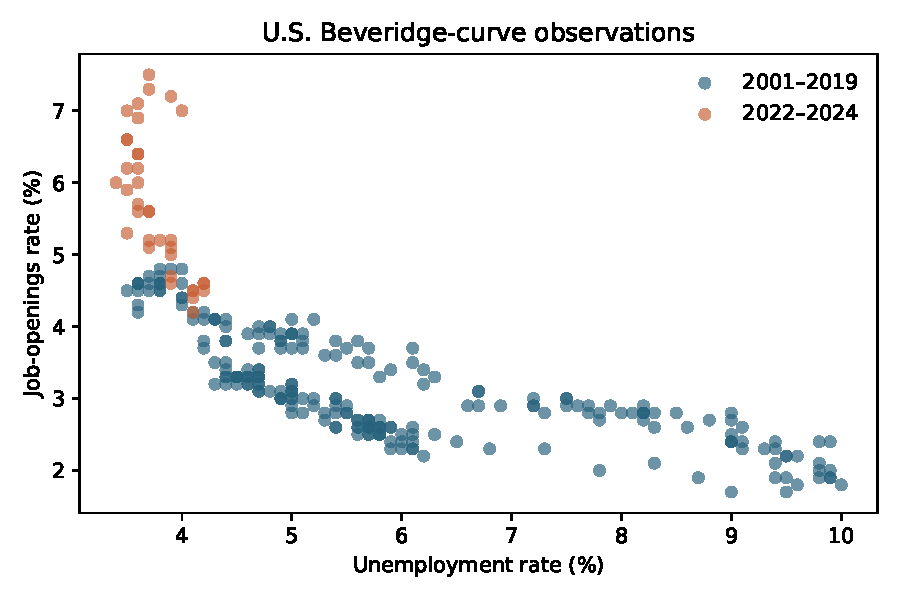
\includegraphics[width=.85\linewidth]{../output/figures/beveridge.pdf}
\caption{Published seasonally adjusted monthly U.S. rates. Each dot is one month. The graph is descriptive and does not fit a structural curve.}
\label{fig:curve}
\end{figure}

\section{Robustness and Failed Persistence Hypothesis}
% [claim:c-normalization]
The same primary-interval calculation for 2024 alone uses \result{last_year_check.n}{12} months. Its mean openings rate was \result{last_year_check.mean}{4.65} percent, only \result{last_year_check.difference_from_pre}{0.55} points above the 2001--2019 conditional mean. Thus the pooled post-2021 difference was much larger than the difference in the final observed year. A trial claim that the 2022 gap remained equally large through 2024 was discarded in the experiment ledger.

\section{Limitations and Interpretation}
% [claim:c-limitations]
The observed conditional difference is not evidence that matching efficiency worsened, a policy caused a shift, or a stable structural curve moved. Vacancy and unemployment measures cover different survey populations; industry mix, recruiting intensity, wages, labor supply, and business-cycle composition can all change their joint distribution. The IMF analysis expresses vacancies relative to the labor force, whereas our BLS openings rate divides openings by employment plus openings; their magnitudes are therefore not directly comparable \citep{KindbergGirard2024}. BLS's JOLTS estimates have sampling and nonsampling error, and histories are revised \citep{BLSJOLTS}. Conditioning on a narrow unemployment interval does not make the unemployment distributions within that interval identical, so the mean gap is not a fixed-unemployment vertical distance. It also does not remove the other confounders. The $[4.0,5.0]$ comparison has just eight post-period months. Annual averages also conceal within-year dynamics. We do not infer statistical significance or extrapolate the 2022--2024 pattern past December 2024. The old and new windows are deliberately different calendar eras, so any difference is descriptive of these selected months only.

\section{Conclusion}
% [claim:c-conclusion]
This pilot reproduces a familiar feature of published U.S. labor-market aggregates: at similar recorded unemployment rates, openings were higher on average in 2022--2024 than in 2001--2019. The gap had narrowed substantially by 2024. The deliverable is a reproducible real-data descriptive note and a tested research package, not a new causal or top-journal contribution.

\section{Reproducibility Appendix}
% [claim:c-design]
The public BLS API was queried in three non-overlapping windows (2001--2010, 2011--2020, 2021--2024). Frozen response bodies, SHA-256 hashes, and acquisition logs are in the \texttt{data/} directory. Running the analysis script from the project root regenerates the panel, results file, table, and figure. The replication configuration specifies a clean isolated replay. The acquisition script refuses to overwrite a prior raw snapshot. This appendix documents computational reproduction of the recorded vintage, not future BLS releases.

\begingroup\scriptsize\setlength{\bibsep}{0pt}
\bibliographystyle{plainnat}
\bibliography{references}
\endgroup
\end{document}
